\subsection{MeZO}
Zeroth-order optimization (ZO-SGD \cite{zo-sgd}) estimates gradients using only forward-passes, making it possible to update neural networks without backpropagation. Memory-efficient Zeroth-order Optimizer (MeZO \cite{mezo})  is an adaptation of the classical zeroth-order optimization method, reducing its memory consumption by operating in-place. This results in a method that is able to fine-tune LMs with the same memory footprint as inference. 
%The authors prove that MeZO can successfully optimize LLMs and show its efficiency 

To estimate gradients, MeZO uses Simultaneous Perturbation Stochastic Approximation (SPSA), which requires two forward passes to estimate the gradient. For each forward pass, the parameters of the model are perturbed by different amounts, depending on a random number sampled for each parameter and the perturbation scale, which is a hyperparameter of the model. For loss function $\mathcal{L}$, model parameters $\mathbf{\theta} \in \mathbb{R}^d$ and minibatch $\mathcal{B}$, SPSA estimates gradient as:

\begin{equation}
    \hat{\nabla}\mathcal{L}(\mathbf{\theta}; \mathcal{B}) = 
    \frac{\mathcal{L}(\mathbf{\theta} + \epsilon\mathbf{z}; \mathcal{B}) - \mathcal{L}(\mathbf{\theta} - \epsilon\mathbf{z}; \mathcal{B})}
    {2 \epsilon} \mathbf{z}
\end{equation}

where $\epsilon$ is the perturbation scale and $\mathbf{z} \in \mathbb{R}^d$ is randomly sampled with $\mathbf{z} \sim \mathcal{N}(0, \textbf{\em I}_d)$. 

Using the SPSA estimate for gradients, the model is updated with SGD:

\begin{equation}
    \mathbf{\theta}_{t+1} = \mathbf{\theta}_t - \eta \hat{\nabla} \mathcal{L}(\mathbf{\theta}; \mathcal{B}_t)
\end{equation}

where $\eta$ is the learning rate. 

MeZO's in-place implementation saves additional memory for this approach. For each batch, MeZO samples a random seed and every time a parameter gets updated or perturbed for the gradient estimation, it samples the random value \textbf{z} using this seed. This way, $\mathbf{z} \in \mathbb{R}^d$ does not need to be stored, theoretically reducing memory consumption to the same as inference. In practice, often entire weight matrices are perturbed instead of individual scalars, saving time but costing additional memory as large as the largest weight matrix. 

\subsubsection{Prompt-based Fine-tuning}

Experiments show that prompting is crucial for the ability of MeZO to optimize the network. Thus, MeZO is used under the prompt-based fine-tuning setting described in \cite{prompt}. 

For each example in the dataset, a model is given a prompt as input; this prompt is a template attached to the input sentence and varies depending on the task and dataset. The template contains a mask token and the model is trained to predict the masked word from a set of label words, where each label word is assigned to one label. Classification is then performed using the logits of the label words on the mask token. \Cref{fig:prompt} shows how prompt-based fine-tuning works on the SST-2 dataset. 

\begin{figure}
    \centering
    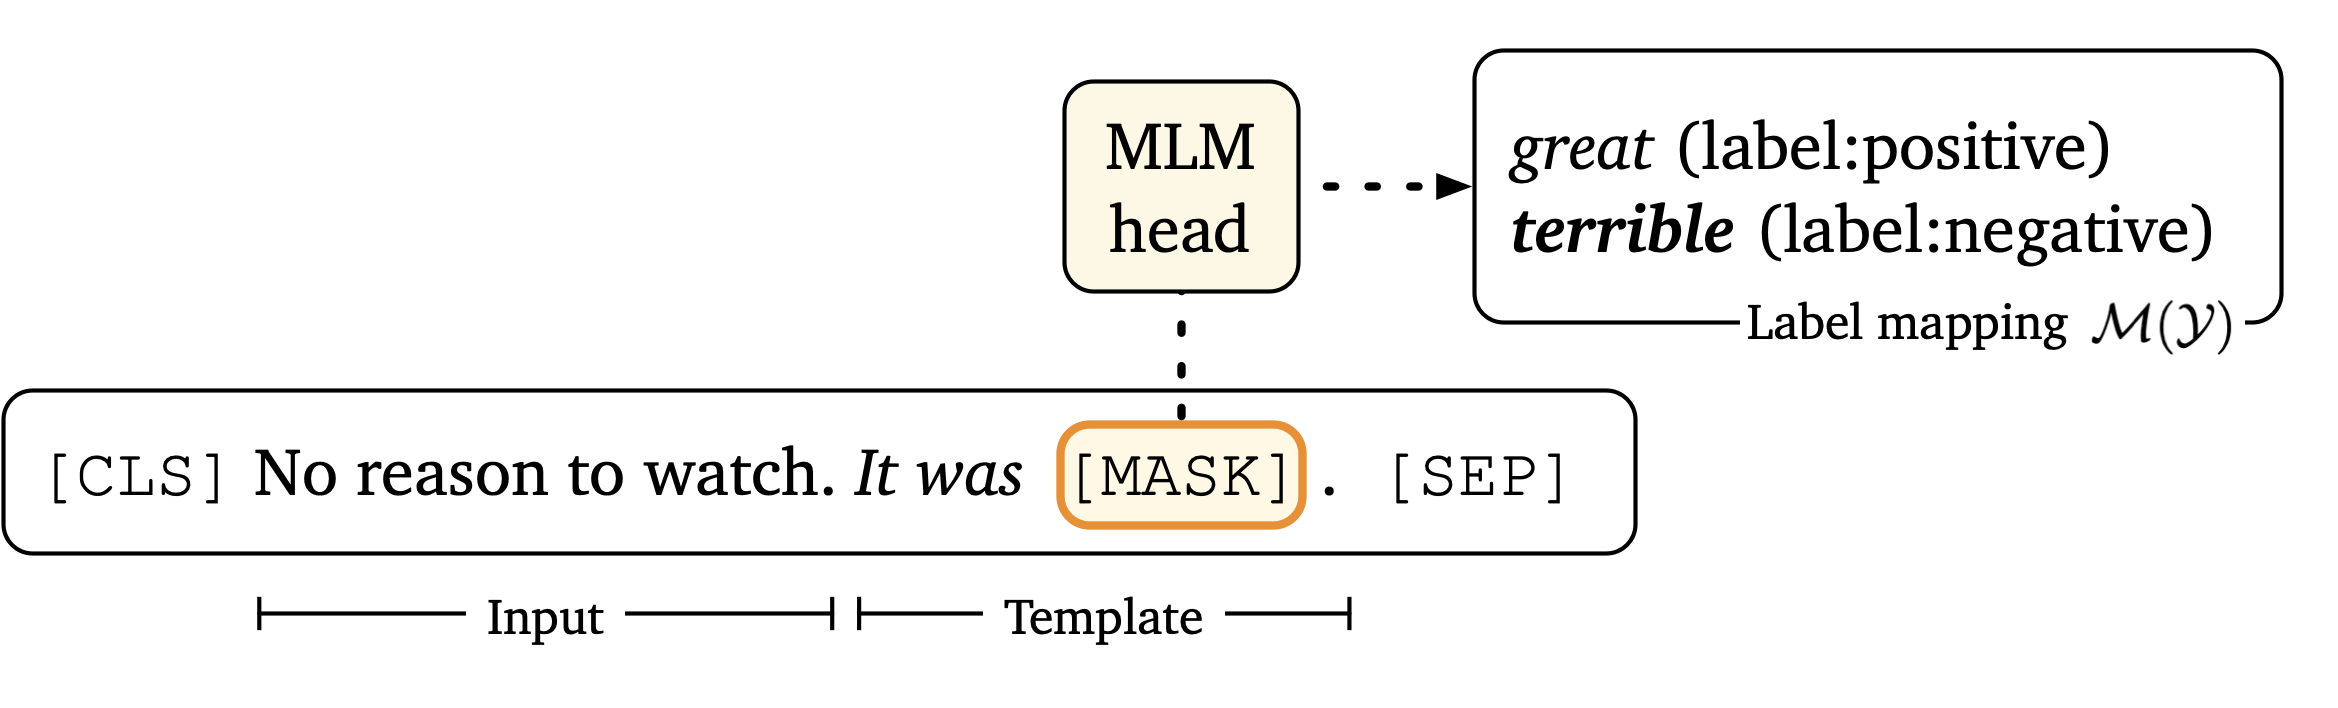
\includegraphics[width=\linewidth]{assets/images/Prompt.png}
    \caption{Prompt-based fine-tuning on SST-2. Adapted from \cite{prompt}. The prompt consists of the input sentence and the template \textit{"It was [MASK]."}. The model is trained to predict the label word \textit{"great"} for positive input sentences and \textit{"terrible"} for negative input sentences.}
    \label{fig:prompt}
\end{figure}